% =====================================================================
%  Artigo - Projeto Integrador de Teoria dos Grafos - Fase I
%  Estudo de caso: Evacuação e Defesa Civil (Córrego do Feijão, Brumadinho-MG)
%  Formatação: modelo SBC (A4, coluna única, Times 12, margens 3,5/2,5/3,0 cm)
%
%  Compilação recomendada:  lualatex artigo.tex   (rodar 2x)
%  Também compila com pdflatex (ex.: Overleaf) - o preâmbulo se adapta.
% =====================================================================
\documentclass[12pt,a4paper]{article}

\usepackage{iftex}
\usepackage[T1]{fontenc}
\usepackage{textcomp}
\usepackage{mathptmx}                   % Times
\usepackage[scaled=.92]{helvet}         % Helvetica (legendas)
\usepackage{courier}
\ifLuaTeX
  \IfFileExists{brazilian.ldf}{%
    \usepackage[brazilian]{babel}%
  }{%
    % Ambiente sem o pacote babel-portuges: usa o .ini do babel e carrega
    % os padrões de hifenização do português (hyph-pt.pat.txt) em tempo real.
    \usepackage[provide=*]{babel}
    \babelprovide[import=pt-BR, main]{brazilian}
    \directlua{
      local f = io.open("hyph-pt.pat.txt")
      if f then
        local p = f:read("*a"); f:close()
        p = p:gsub("\string\n", " ")
        tex.print("\string\\babelpatterns[brazilian]{" .. p .. "}")
      end
    }%
  }
\else
  \usepackage[utf8]{inputenc}
  \usepackage[brazilian]{babel}
\fi

\usepackage[a4paper,top=3.5cm,bottom=2.5cm,left=3cm,right=3cm]{geometry}
\usepackage{graphicx}
\usepackage{amsmath}
\usepackage{booktabs}
\usepackage{array}
\usepackage{enumitem}
\usepackage{microtype}
\usepackage[hidelinks]{hyperref}
\usepackage{url}
\urlstyle{same}

% ---------------- Estilo SBC ----------------
\pagestyle{empty}                       % sem cabeçalho, rodapé e numeração
\setlength{\parindent}{1.27cm}          % recuo dos parágrafos subsequentes
\setlength{\parskip}{6pt}               % 6 pt antes de cada parágrafo
\frenchspacing
\sloppy

\makeatletter
% Seções: negrito 13 pt, alinhadas à esquerda, 12 pt extras antes
\renewcommand\section{\@startsection{section}{1}{\z@}%
  {12pt}{0.1pt}{\normalfont\fontsize{13}{15}\selectfont\bfseries}}
% Subseções: negrito 12 pt
\renewcommand\subsection{\@startsection{subsection}{2}{\z@}%
  {12pt}{0.1pt}{\normalfont\normalsize\bfseries}}
\renewcommand\thesection{\arabic{section}.}
\renewcommand\thesubsection{\arabic{section}.\arabic{subsection}.}
\renewcommand\@seccntformat[1]{\csname the#1\endcsname\ }
\makeatother

% Legendas: Helvetica 10 pt negrito; centralizadas se tiverem uma linha,
% justificadas com recuo de 0,8 cm caso contrário; 6 pt antes e depois.
\usepackage[font={sf,bf,footnotesize},labelsep=period,justification=justified,
            singlelinecheck=true,margin=0.8cm,skip=6pt]{caption}
\captionsetup[table]{position=top}
\setlength{\abovecaptionskip}{6pt}
\setlength{\belowcaptionskip}{6pt}
\addto\captionsbrazilian{\renewcommand{\tablename}{Tabela}\renewcommand{\figurename}{Figura}}

% Resumo / Abstract: Times 12, recuo de 0,8 cm nas duas margens
\newenvironment{sbcabstract}[1]%
  {\list{}{\leftmargin=0.8cm\rightmargin=0.8cm\topsep=0pt\parsep=0pt}\item[]\textbf{#1.}\ }%
  {\endlist}

% Referências: 12 pt, 6 pt antes de cada uma, recuo de 0,5 cm nas linhas seguintes
\newenvironment{referencias}%
  {\section*{Referências}\begin{list}{}{\leftmargin=0.5cm\itemindent=-0.5cm%
   \labelwidth=0pt\labelsep=0pt\itemsep=0pt\parsep=0pt\topsep=0pt}\setlength{\parskip}{6pt}}%
  {\end{list}}
\newcommand{\referencia}{\item\relax}

\newcommand{\us}{\,\textmu s}


% =====================================================================
\begin{document}
% SBC: o primeiro parágrafo de cada seção não tem recuo (o babel em português o ativaria)
\makeatletter\let\@afterindenttrue\@afterindentfalse\makeatother

\begin{center}
  \vspace*{12pt}
  {\fontsize{16}{19}\selectfont\bfseries
   Vias Críticas e Conectividade da Malha Viária de Córrego do Feijão (Brumadinho--MG): uma Análise com Teoria dos Grafos\par}
  \vspace{12pt}
  {\bfseries Caroline Lopes Martins, Ian Melo Gonçalves, Matheus Filipe da Silva Ponte, Guilherme Amaro de Castro, Bruno Nobrega Souza\par}
  \vspace{12pt}
  Curso de Ciência da Computação -- Centro Universitário IESB, Campus Asa Sul\\ Brasília -- DF -- Brasil\par
\end{center}

\begin{sbcabstract}{Abstract}
This paper models the road network around the Córrego do Feijão mine (Brumadinho, Brazil), site of the 2019 B1 dam collapse, as a graph built from OpenStreetMap data (3,143 vertices, 3,199 edges). Author-written C implementations of BFS, DFS, connected components, cycle detection and Tarjan's algorithm show that 50.5\% of the edges are bridges and that 145 of 351 road stretches have no alternative route. Stress tests confirm linear growth of the traversals, expose a quadratic bottleneck in one implementation and measure a 310-fold memory gap between adjacency matrix and list.
\end{sbcabstract}

\begin{sbcabstract}{Resumo}
Este artigo modela a malha viária do entorno da mina Córrego do Feijão (Brumadinho--MG), onde a barragem B1 se rompeu em 2019, como um grafo obtido do OpenStreetMap (3.143 vértices e 3.199 arestas). Implementações autorais em C de BFS, DFS, componentes conexos, detecção de ciclos e do algoritmo de Tarjan mostram que 50,5\% das arestas são pontes e que 145 de 351 trechos viários não têm rota alternativa. Testes de estresse confirmam o crescimento linear das buscas, expõem um gargalo quadrático em uma implementação e medem uma diferença de 310 vezes no consumo de memória entre matriz e lista de adjacência.
\end{sbcabstract}

% ---------------------------------------------------------------------
\section{Introdução}

Em 25 de janeiro de 2019, a barragem B1 da mina Córrego do Feijão, em Brumadinho (MG), rompeu-se e liberou mais de 11 milhões de m$^3$ de rejeitos, que percorreram cerca de 10\,km e deixaram 259 mortos e 11 desaparecidos até janeiro de 2020 [Rotta et al. 2020]. Após o desastre, a Política Nacional de Segurança de Barragens passou a exigir a delimitação da Zona de Autossalvamento, o trecho a jusante em que não há tempo para a intervenção das autoridades [Brasil 2020]. Nessa zona, a população precisa sair por conta própria, e a \emph{estrutura} da malha viária torna-se uma questão de segurança: uma comunidade ligada ao restante da rede por uma única estrada fica isolada se esse trecho for atingido.

Modelando cruzamentos como vértices e vias como arestas, perguntas da Defesa Civil tornam-se propriedades de um grafo: \emph{quais regiões estão desconectadas?} (componentes conexos), \emph{quais vias não têm desvio?} (pontes), \emph{quais cruzamentos, se bloqueados, partem a rede?} (vértices de articulação) e \emph{em que ordem a frente de rejeitos alcança cada ponto?} (níveis de uma busca em largura). Este trabalho, correspondente à Fase I do projeto, trata dessas questões de topologia, sem pesos nas arestas. As contribuições são: (i) a construção de um grafo real da região a partir de dados abertos; (ii) a implementação autoral em C das representações por lista e por matriz de adjacência e de seis análises estruturais; (iii) a identificação das vias críticas da região; e (iv) uma avaliação experimental de tempo e memória que verifica as complexidades teóricas. As Seções~2 a 5 apresentam, respectivamente, os trabalhos relacionados, a metodologia, os resultados e a conclusão.

% ---------------------------------------------------------------------
\section{Trabalhos Relacionados}

Porta, Crucitti e Latora [Porta et al. 2006] formalizaram a abordagem primal para redes de ruas, em que interseções são vértices e segmentos são arestas, convenção adotada aqui. A biblioteca OSMnx [Boeing 2017] automatiza a construção desses grafos a partir do OpenStreetMap e simplifica os pontos de geometria que não são cruzamentos, tema que reaparece na Seção~4. Quanto à vulnerabilidade, Jenelius, Petersen e Mattsson [Jenelius et al. 2006] distinguem a importância de um enlace da exposição de uma região e mostram que áreas rurais esparsas são as mais expostas, enquanto Sullivan et al. [Sullivan et al. 2010] estudam os \emph{enlaces isoladores}, cuja remoção desconecta a rede, ou seja, as pontes no sentido da Teoria dos Grafos. Modelos de evacuação por fluxo em redes [Hamacher and Tjandra 2002] pressupõem a topologia conhecida, o que esta Fase I fornece. Os algoritmos de busca e suas aplicações seguem [Cormen et al. 2009], e a detecção de pontes e articulações em tempo linear com uma única DFS deve-se a Tarjan [Tarjan 1972]. Diferentemente desses trabalhos, aqui os algoritmos são implementados do zero e o custo de cada decisão de implementação é medido.

% ---------------------------------------------------------------------
\section{Metodologia e Modelagem}

\subsection{Base de dados e modelagem}

Os dados foram extraídos do OpenStreetMap [OpenStreetMap contributors 2026] via \emph{overpass-turbo}, em GeoJSON. A área cobre cerca de 6,9\,km\,$\times$\,5,5\,km ao redor da mina, incluindo a comunidade de Córrego do Feijão. O arquivo contém 224 vias descritas por 3.423 pares de coordenadas; predominam vias de serviço (69), estradas rurais não pavimentadas (57), vias terciárias (30) e trilhas (29), o que caracteriza uma malha rural.

O grafo $G=(V,E)$ é \textbf{não direcionado e não ponderado}: numa evacuação, as vias são percorridas nos dois sentidos, e a Fase I trata apenas de conectividade. Cada coordenada distinta é um vértice e cada par de coordenadas consecutivas de uma via é uma aresta; vias que compartilham uma coordenada compartilham o vértice, o que conecta a rede nos cruzamentos. Um \emph{parser} GeoJSON próprio localiza cada coordenada por busca linear com tolerância de $10^{-7}$ graus e descarta laços e arestas repetidas. O resultado tem $|V| = 3.143$ vértices e $|E| = 3.199$ arestas, somando 88,3\,km de vias (comprimento pela fórmula de Haversine).

A estrutura \texttt{Grafo} mantém simultaneamente uma \textbf{lista de adjacência} (vetor de listas encadeadas com nós de 16 bytes) e uma \textbf{matriz de adjacência} de inteiros, ambas com crescimento por duplicação de capacidade. Em 64 bits, a memória exata de cada representação é
\begin{equation}
M_{\text{lista}} = 8|V| + 32|E| \qquad\text{e}\qquad M_{\text{matriz}} = 8|V| + 4|V|^2 \text{ bytes.}
\label{eq:memoria}
\end{equation}

\subsection{Algoritmos}

Os algoritmos foram escritos em C sem bibliotecas de grafos, com fila circular própria e um módulo de \emph{log} que registra tempo (ms) e memória de cada execução. \textbf{BFS} e \textbf{DFS} (recursiva) são a base das demais análises. Os \textbf{componentes conexos} são obtidos repetindo a BFS a partir de cada vértice ainda não visitado. A \textbf{detecção de ciclos e bipartição} usa uma BFS que colore os vértices com duas cores alternadas: uma aresta para um vértice já visitado que não seja o pai indica ciclo, e extremos de mesma cor indicam que o grafo não é bipartido. A \textbf{propagação} parte do vértice mais próximo da barragem B1 (20\textdegree07'11''S, 44\textdegree07'17''W) e usa o nível da BFS como unidade discreta de tempo. O \textbf{algoritmo de Tarjan} faz uma DFS que registra o instante de descoberta $d[v]$ e o menor instante $low[v]$ alcançável pela subárvore de $v$ com uma aresta de retorno; a aresta $(u,v)$ é ponte se $low[v] > d[u]$, e $u$ é articulação se $low[v] \ge d[u]$ para algum filho $v$ (ou se $u$ for raiz com dois ou mais filhos). Todos têm complexidade $O(|V|+|E|)$ com lista de adjacência.

\subsection{Protocolo experimental}

Os testes de estresse usaram subgrafos conexos com 100, 250, 500, 1.000, 1.500, 2.000 e 2.500 vértices, além do grafo completo, cada um induzido pelos $N$ primeiros vértices de uma BFS a partir do vértice 0 (os de 100, 500 e 1.000 vértices coincidem com os CSV do repositório). Como cada execução dura microssegundos, o algoritmo é repetido $R$ vezes, com $R$ calibrado para o lote durar ao menos 20\,ms; reporta-se a mediana de 11 lotes, medida com relógio monotônico e com a escrita do \emph{log} em disco desativada. Para comparar as representações também em tempo, incluiu-se uma variante da BFS que percorre a matriz. Ambiente: Intel Xeon 2,1\,GHz, Linux e GCC 13.3 (\texttt{-O2}). Os resultados estruturais foram validados de forma independente com a biblioteca NetworkX 3.6 [Hagberg et al. 2008] sobre a mesma lista de arestas e coincidiram integralmente.

% ---------------------------------------------------------------------
\section{Resultados e Discussão}

\subsection{Estrutura da malha viária}

A Tabela~\ref{tab:estrutura} resume as propriedades do grafo. O grau médio de 2,04 e a densidade de 0,065\% indicam uma rede muito esparsa. A distribuição de graus é reveladora: 2.848 vértices (90,6\%) têm grau 2, ou seja, não são cruzamentos, mas pontos que descrevem a curvatura das estradas; apenas 193 vértices têm grau 3 ou mais, e 102 são finais de via.

\begin{table}[!htb]
\caption{Propriedades estruturais do grafo de Córrego do Feijão.}
\label{tab:estrutura}
\centering\small
\begin{tabular}{@{}lr@{\hspace{0.6cm}}lr@{}}
\toprule
\textbf{Propriedade} & \textbf{Valor} & \textbf{Propriedade} & \textbf{Valor}\\
\midrule
Vértices / arestas & 3.143 / 3.199 & Pontes & 1.615 (50,5\%)\\
Extensão das vias & 88,3\,km & Extensão em pontes & 46,0\,km (52,1\%)\\
Grau médio / máximo & 2,04 / 5 & Trechos-ponte / trechos & 145 / 351\\
Componentes conexos & 3 & Vértices de articulação & 1.577\\
Maior componente & 3.115 vértices & \quad dos quais com grau $\ge 3$ & 107\\
Possui ciclo / é bipartido & sim / não & Número ciclomático & 59\\
\bottomrule
\end{tabular}
\end{table}

\textbf{Componentes, ciclos e bipartição.} Há três componentes: o principal, com 3.115 vértices, e dois fragmentos de 15 e 13 vértices sem ligação com a rede mapeada, que devem ser verificados em campo (conexão ausente no mapa ou acesso apenas por fora da área). A rede tem ciclos e não é bipartida, mas o número ciclomático $|E|-|V|+c$, que conta os ciclos independentes, é apenas 59 para mais de 3 mil arestas: a malha é quase uma árvore.

\textbf{Pontes e articulações.} Esse caráter arbóreo explica o principal achado: 1.615 arestas (50,5\%) são pontes, cobrindo 52,1\% da extensão viária. Como uma única estrada gera dezenas de pontes consecutivas, os resultados foram agregados em \emph{trechos}, sequências de arestas entre vértices de grau diferente de 2. Dos 351 trechos, \textbf{145 são vias críticas}: a interdição de qualquer ponto delas isola parte da comunidade. Dos 1.577 vértices de articulação, apenas 107 são cruzamentos reais, candidatos prioritários a reforço estrutural e pré-posicionamento de equipes. A Figura~\ref{fig:mapa}(a) mostra que as pontes formam ramificações sem saída a partir de um núcleo com rotas redundantes; removidas as pontes, restam nove núcleos 2-aresta-conexos, o maior com 1.286 vértices. O resultado confirma, para Córrego do Feijão, que redes rurais esparsas são as mais expostas a falhas pontuais [Jenelius et al. 2006].

\begin{figure}[!htb]
\centering
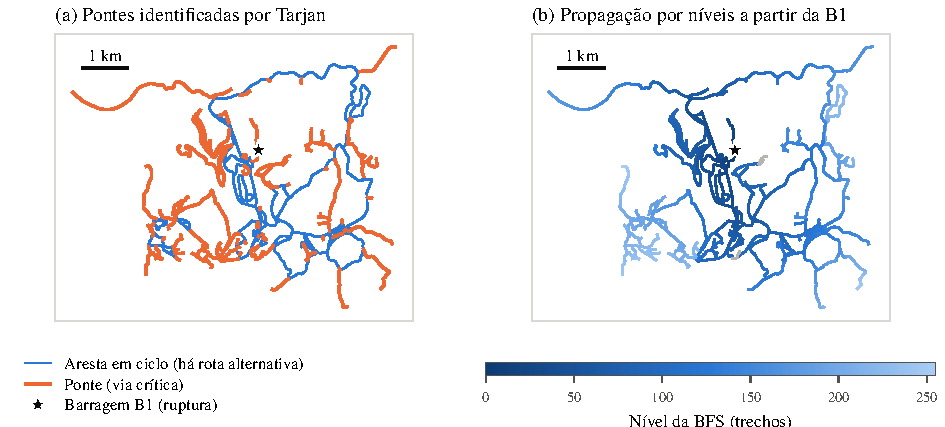
\includegraphics[width=0.86\textwidth]{figuras/mapa.pdf}
\caption{(a) Pontes identificadas pelo algoritmo de Tarjan (laranja) e arestas em ciclos (azul). (b) Nível da BFS a partir do vértice mais próximo da barragem B1; em cinza, os componentes desconectados.}
\label{fig:mapa}
\end{figure}

\begin{figure}[!htb]
\centering
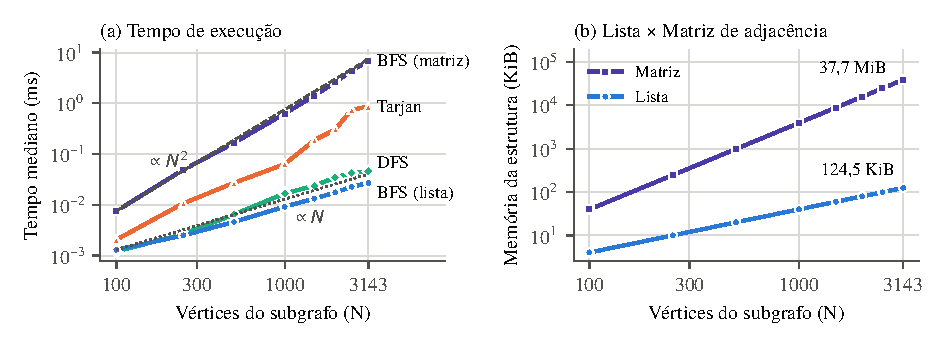
\includegraphics[width=0.94\textwidth]{figuras/desempenho.pdf}
\caption{(a) Tempo mediano de execução (log-log); tracejado: crescimento $\propto N$ e $\propto N^2$; Tarjan na versão original. (b) Memória das duas representações.}
\label{fig:desempenho}
\end{figure}

\textbf{Propagação a partir da B1.} O vértice mais próximo da barragem está a 126,9\,m dela; a BFS a partir dele alcança os 3.115 vértices do componente principal, com excentricidade de 256 níveis (Figura~\ref{fig:mapa}(b)). Até o nível 25 são alcançados 94 vértices, e até o nível 50, 310 (10\% da rede). Como 90,6\% dos vértices são pontos de geometria, o nível mede segmentos digitalizados e não distância: uma estrada sinuosa recebe mais níveis que uma reta de mesmo comprimento. O resultado ordena alertas, mas estimar \emph{tempo} de chegada exige pesos (Fase II).

\subsection{Desempenho e consumo de memória}

A Figura~\ref{fig:desempenho} e a Tabela~\ref{tab:tempos} apresentam os testes de estresse, com o expoente $k$ de $T(N) \approx c\,N^k$ ajustado em escala log-log para $N \ge 500$. BFS, DFS, componentes, ciclos e propagação têm $k$ entre 0,93 e 1,09, compatível com $O(|V|+|E|)$, já que $|E|$ fica entre $1{,}02\,|V|$ e $1{,}05\,|V|$ em todos os subgrafos. A BFS percorre o grafo completo em 27,1\us; a DFS é 1,7 vez mais lenta, custo atribuível às chamadas recursivas.


\begin{table}[!htb]
\caption{Tempo mediano por execução (\textmu s) e expoente empírico $k$.}
\label{tab:tempos}
\centering\small
\begin{tabular}{@{}lrrrrr@{}}
\toprule
\textbf{Algoritmo} & $N=100$ & $N=500$ & $N=1.000$ & $N=3.143$ & $k$\\
\midrule
BFS (lista de adjacência)  & 1,3 & 4,6 & 9,2 & 27,1 & 0,97\\
DFS                        & 1,2 & 6,5 & 16,8 & 45,5 & 1,09\\
Componentes conexos        & 2,0 & 6,1 & 11,4 & 43,0 & 1,01\\
Ciclos e bipartição        & 1,3 & 4,6 & 9,4 & 26,5 & 0,93\\
Propagação (BFS por níveis)& 1,9 & 5,6 & 10,2 & 29,5 & 0,93\\
Tarjan (implementação original) & 2,1 & 27,0 & 63,5 & 860,4 & 2,01\\
Tarjan (com vetor de marcação)  & 1,2 & 8,2 & 18,8 & 59,9 & 1,12\\
BFS (matriz de adjacência) & 7,6 & 166,1 & 627,3 & 6.910,9 & 2,04\\
\bottomrule
\end{tabular}
\end{table}

\textbf{Gargalo no algoritmo de Tarjan.} A implementação original teve $k = 2{,}01$, embora o algoritmo seja linear. A causa está na função que evita registrar uma articulação duas vezes: ela percorre a lista de articulações já encontradas, com custo $O(A)$ por consulta. Como aqui $A \approx |V|/2$, o total torna-se $O(|V|^2)$. Com um vetor booleano de marcação (consulta $O(1)$), o tempo no grafo completo caiu de 860,4 para 59,9\us\ (14 vezes) e $k$ voltou a 1,12, com resultados idênticos. A complexidade teórica só se mantém se as estruturas auxiliares também a respeitam, e foi a medição que revelou o problema.

\textbf{Lista \emph{versus} matriz.} Os valores medidos seguem a Equação~\ref{eq:memoria}: com $|E| \approx |V|$, a lista cresce linearmente e a matriz, quadraticamente. A razão entre elas passa de 9,8 vezes com 100 vértices (40.800 contra 4.160 bytes) para 310 vezes no grafo completo (37,7\,MiB contra 124,5\,KiB). Na carga real o custo é maior, pois a matriz é alocada pela capacidade: o crescimento por duplicação reserva uma matriz $4.096 \times 4.096$ (64\,MiB), com 99,96\% de zeros. No tempo, a BFS sobre a matriz varre uma linha inteira por vértice, tem $k = 2{,}04$ e é 255 vezes mais lenta que sobre a lista no grafo completo. A matriz só compensaria em grafos densos ou se a consulta $O(1)$ de adjacência dominasse, o que aqui ocorre apenas ao descartar arestas repetidas.

Por fim, a leitura do GeoJSON levou 19,7\,ms (mediana de 15 execuções), mais que qualquer análise, porque a busca linear de vértices a torna $O(P \cdot |V|)$ para $P = 3.423$ pontos; uma tabela \emph{hash} sobre as coordenadas a tornaria linear.

% ---------------------------------------------------------------------
\section{Conclusão e Trabalhos Futuros}

A malha viária de Córrego do Feijão é esparsa, quase arbórea e frágil: metade das arestas são pontes, 145 trechos não têm rota alternativa e 107 cruzamentos são pontos únicos de falha, o que dá à Defesa Civil uma lista objetiva de prioridades para reforço preventivo. Os experimentos confirmaram o crescimento linear das buscas, mostraram que a lista de adjacência é a representação adequada para redes viárias e revelaram, por medição, um gargalo quadrático na implementação de Tarjan.

Na Fase II, as arestas receberão pesos pela distância de Haversine, o algoritmo de Dijkstra calculará rotas seguras até áreas de refúgio e a Cobertura de Vértices orientará o posicionamento de postos de socorro. A contração dos vértices de grau 2 reduzirá o grafo a 295 vértices e 351 arestas sem alterar sua conectividade.

% ---------------------------------------------------------------------
\begin{referencias}
\referencia Boeing, G. (2017). OSMnx: New methods for acquiring, constructing, analyzing, and visualizing complex street networks. \emph{Computers, Environment and Urban Systems}, 65:126--139.

\referencia Brasil (2020). Lei n\textordmasculine{} 14.066, de 30 de setembro de 2020. Altera a Política Nacional de Segurança de Barragens (Lei n\textordmasculine{} 12.334/2010). \emph{Diário Oficial da União}.

\referencia Cormen, T. H., Leiserson, C. E., Rivest, R. L. and Stein, C. (2009). \emph{Introduction to Algorithms}. MIT Press, 3rd edition.

\referencia Hagberg, A. A., Schult, D. A. and Swart, P. J. (2008). Exploring network structure, dynamics, and function using NetworkX. In \emph{Proc. 7th Python in Science Conference}, pages 11--15.

\referencia Hamacher, H. W. and Tjandra, S. A. (2002). Mathematical modelling of evacuation problems: a state of the art. In \emph{Pedestrian and Evacuation Dynamics}, pages 227--266. Springer.

\referencia Jenelius, E., Petersen, T. and Mattsson, L.-G. (2006). Importance and exposure in road network vulnerability analysis. \emph{Transportation Research Part A}, 40(7):537--560.

\referencia OpenStreetMap contributors (2026). Dados extraídos via overpass-turbo em 8 set. 2026 (licença ODbL). \url{https://www.openstreetmap.org}.

\referencia Porta, S., Crucitti, P. and Latora, V. (2006). The network analysis of urban streets: a primal approach. \emph{Environment and Planning B}, 33(5):705--725.

\referencia Rotta, L. H. S. et al. (2020). The 2019 Brumadinho tailings dam collapse: Possible cause and impacts of the worst human and environmental disaster in Brazil. \emph{International Journal of Applied Earth Observation and Geoinformation}, 90:102119.

\referencia Sullivan, J. L., Novak, D. C., Aultman-Hall, L. and Scott, D. M. (2010). Identifying critical road segments and measuring system-wide robustness in transportation networks with isolating links. \emph{Transportation Research Part A}, 44(5):323--336.

\referencia Tarjan, R. (1972). Depth-first search and linear graph algorithms. \emph{SIAM Journal on Computing}, 1(2):146--160.
\end{referencias}

\end{document}
